\chapter{Perspective on Efficiency}
The code written for this project was not designed to be efficient,
but to be understandable to the reader and the authors,
because efficiency was outside the scope of the project.

In a real world scenario,
efficiency both in time and power consumption is crucial to the effectiveness of a rescue robot.

Because of this we want to at least formulate our thoughts on the topic.
\section{Pathfinding}
Pathfinding is probably the most resource-heavy calculation in our system,
and will likely be executed several times while running.
ction
Most pathfinding algorithms need several variables to be stored and accessed multiple times,
for each node.
We decided to store them in structs for our implementation.

\lstinputlisting
[firstline=24,				%starts reading the file from this line
firstnumber=24,
lastline=31,
label=lst:structs,	%label
caption={Declaring a Struct  in {\tt defs.h}}
]{code/defs.h}
%
An example of a struct declaration can be seen in Listing \ref{lst:structs}.
A struct stores all declared variables as an individual variable,
with pointers to them.
This makes it easy to access them for the programmer,
but creates a notable overhead when compiling.

Depending on the word size of the used processor,
it could be possible to store all information necessary for a node in one variable.
This would necessitate inventing a custom encoding,
but would possibly improve time consumption on runtime.

One idea for this would be to reserve sections of the variables bits for specific information,
our thoughts on how that might look can be seen in Table \ref{tab:encode}.

\begin{table}[h]
\caption{Example of a possible custom Encoding for Nodes}
\begin{tabularx}{\textwidth}{|*{32}{X|}}
	\hline
	\multicolumn{8}{|>{\hsize=\dimexpr2\hsize+2\tabcolsep+\arrayrulewidth\relax}X|}{position}&
	\multicolumn{8}{>{\hsize=\dimexpr2\hsize+2\tabcolsep+\arrayrulewidth\relax}X|}{walls}&
	\multicolumn{8}{>{\hsize=\dimexpr2\hsize+2\tabcolsep+\arrayrulewidth\relax}X|}{parent}&
	\multicolumn{8}{>{\hsize=\dimexpr8\hsize+10\tabcolsep+\arrayrulewidth\relax}X|}{movecost}\\
	\hline
	1&1&0&1&1&0&0&1&0&1&0&1&1&0&0&0&0&1&1&1&0&0&1&0&1&0&1&1&1&1&1&1\\
	\hline
\end{tabularx}
\label{tab:encode}
\end{table}
%
Single values could be retrieved through simple bitwise operations,
implemented either in hardware or in software.
To retrieve the position for example,
the whole value could be shifted to the right 24 times.

To select the parent position,
one could take the value {\tt AND} {\tt 0xFF00} and
afterwards shift to the right 8 times.

This would make it possible to store the newly invented variables in a 2D array,
like we do now with our {\tt node struct}.
But since we would refer to every node as its position,
we would only need to make single array lookups,
instead of multiple pointer lookups.

Our current approach takes use of pointers a lot,
often iterating through several substructs.
Listing \ref{lst:pointer_access} shows code with multiple pointer accesses per line.
Code similar to this listing gets executed up to 8 times per \emph{node},
for every \emph{node} with a lower \emph{cost to reach} than the finish \emph{node},
to check for every direction whether moving there would be shorter.

\lstinputlisting
[firstline=84,				%starts reading the file from this line
firstnumber=84,
lastline=88,
label=lst:pointer_access,	%label
caption={Accessing several Fields through multiple Pointers in {\tt path.c}}
]{code/path.c}
%
When implementing Dijkstra's algorithm or A*,
there is no need to look at an already checked \emph{node}.
It could therefore be an option to remove all pointers to a node,
when pushing it to the checked stack.

In our current implementation,
those pointers can only be set to {\tt NULL} after finding them through another pointer lookup.
We are already doing this in line 87 in Listing \ref{lst:pointer_access},
when removing the reference to the parent as a neighbour,
to remove redundant information and ease the lookup procedure.

The whole part of linking the \emph{nodes} to their neighbours,
as shown in \ref{lst:linkingByte},
uses the aforementioned {\tt walls} byte,
to compute in what directions to link.
This means that basically the neighbours are stored redundantly,
once in the {\tt walls} byte and once in the eight pointers.

\lstinputlisting
[firstline=7,				%starts reading the file from this line
firstnumber=7,
lastline=20,
label=lst:linkingByte,	%label
caption={Linking Nodes based on {\tt walls} variable in {\tt path.c}}
]{code/path.c}
%

\section{Scan}
When developing the {\tt scan} function,
we had already thought about efficiency to some extend.
Our robot was designed specifically to move in eight directions,
so we could store the information about each \emph{node} in one byte.

We therefore designed the function to return one byte value,
representing the environment at the current position.

We didn't have the opportunity to finalise our idea,
since we had troubles acquiring functioning sensors,
and only used hardcoded values for testing.

\section{Map Handling}
Our approach to map handling was also mainly focused on usability,
not on efficiency.

We also think, that this specific subsystem needs to be very fail-safe,
and therefore persistent.
Without the map handling,
the robot can't keep track of its current position,
which it also should be able to find again after losing power.

Listing \ref{lst:loadingMap} shows our current approach to knowing the map size.

\lstinputlisting
[firstline=31,				%starts reading the file from this line
firstnumber=31,
lastline=46,
label=lst:loadingMap,	%label
caption={Loading the Map from a File in {\tt map.c}}
]{code/map.c}
%
We are reading the file twice,
counting the characters and the lines first and storing the map content in the second iteration.

This could for example be prevented through the user inputting the map size manually,
or storing the dimensions in the header of the map file.

\lstinputlisting
[firstline=105,				%starts reading the file from this line
firstnumber=105,
lastline=123,
label=lst:loadingNodeMap,	%label
caption={Loading the Node Map from the stored Map in {\tt map.c}}
]{code/map.c}
%
After loading the map into memory,
we have to convert the text into a node map.
This process happens in two nested {\tt for loop}s, as can be seen in Listing \ref{lst:loadingNodeMap}.

For a final, more efficient solution,
we would want to store the map in a format ready for import,
and have all conversion happen on the users computer.

The scope of the project didn't allow us to develop a file format and external program to do this,
but we strongly believe,
that it would make the map handling more efficient.

\section{Movement}
Because the movement subsystem was developed very close to hardware level,
we believe that it already is fairly efficient.
We therefore want to highlight the measures we took,
to ensure this.

All four motors get controlled by a single stepping sequence,
not only making them run synchronously,
but also necessitating less interrupts than stepping them individually.
Subsection \ref{sub:circuit} explains the circuit we developed,
to make this possible.

\lstinputlisting
[firstline=13,				%starts reading the file from this line
firstnumber=13,
lastline=28,
label=lst:Stepping,	%label
caption={Part of the {\tt stepping} function in {\tt movement.c}}
]{code/movement.c}
%
The stepping shown in Listing \ref{lst:Stepping} mainly relies on the timer circuits in the microcontroller,
which are accessible also in most powered down modes.

We also believe, that it would be possible and fairly easy,
to implement this behaviour using sequential logic,
in which way it could run directly off an external clock source.
Our thoughts on what that might look like are depicted in Figure \ref{fig:sequential}.

\begin{figure}[hp]
	\centering
	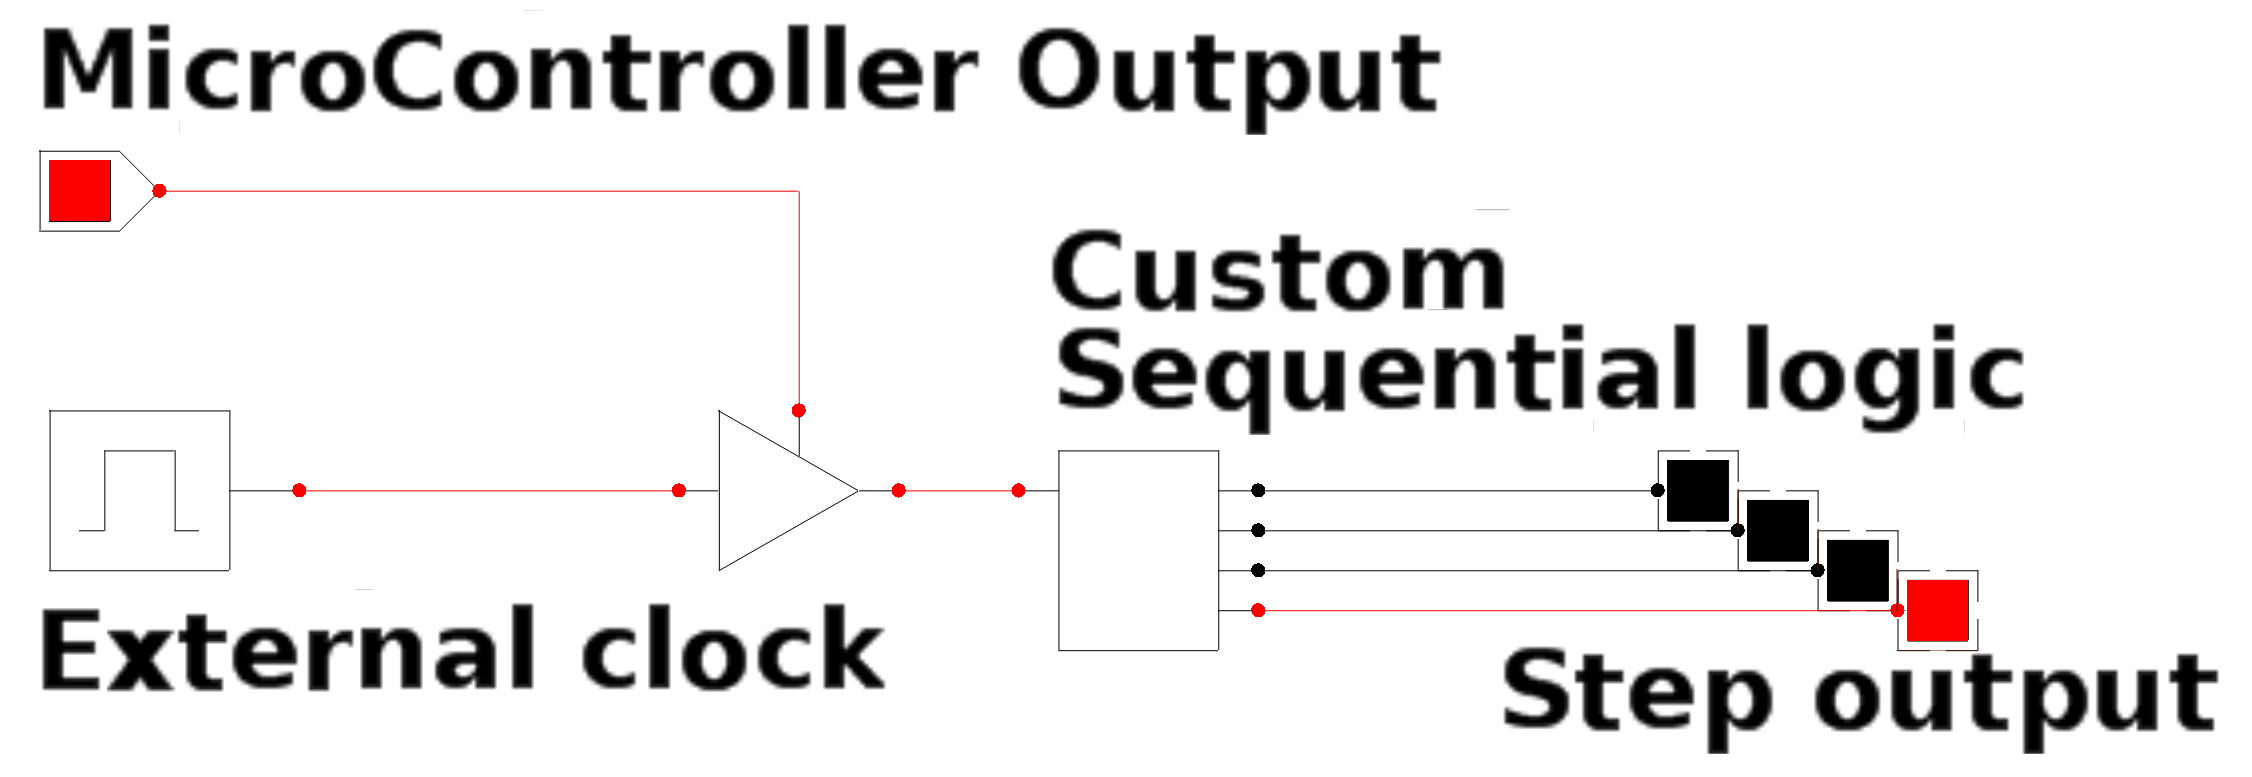
\includegraphics[width=0.8\textwidth]{figures/move/sequential_logic}
	\caption{Mock-up of a sequential stepping Solution}
	\label{fig:sequential}
\end{figure}
%